
\documentclass[11pt, a4paper]{article}
\usepackage[a4paper, margin=1in]{geometry}
\usepackage{tikz}
\usepackage{fontspec}
\usepackage[english]{babel}
\usepackage{longtable} 
\usepackage{booktabs}

% Use Noto Sans for clean, modern look
\babelfont{rm}{Noto Sans} 

% FIXED: Loaded 'babel' library to prevent conflicts with TikZ syntax
\usetikzlibrary{mindmap, trees, shadows, babel}

\pagestyle{empty} 

\begin{document}
\centering
\section*{Project Phases Mind Map}

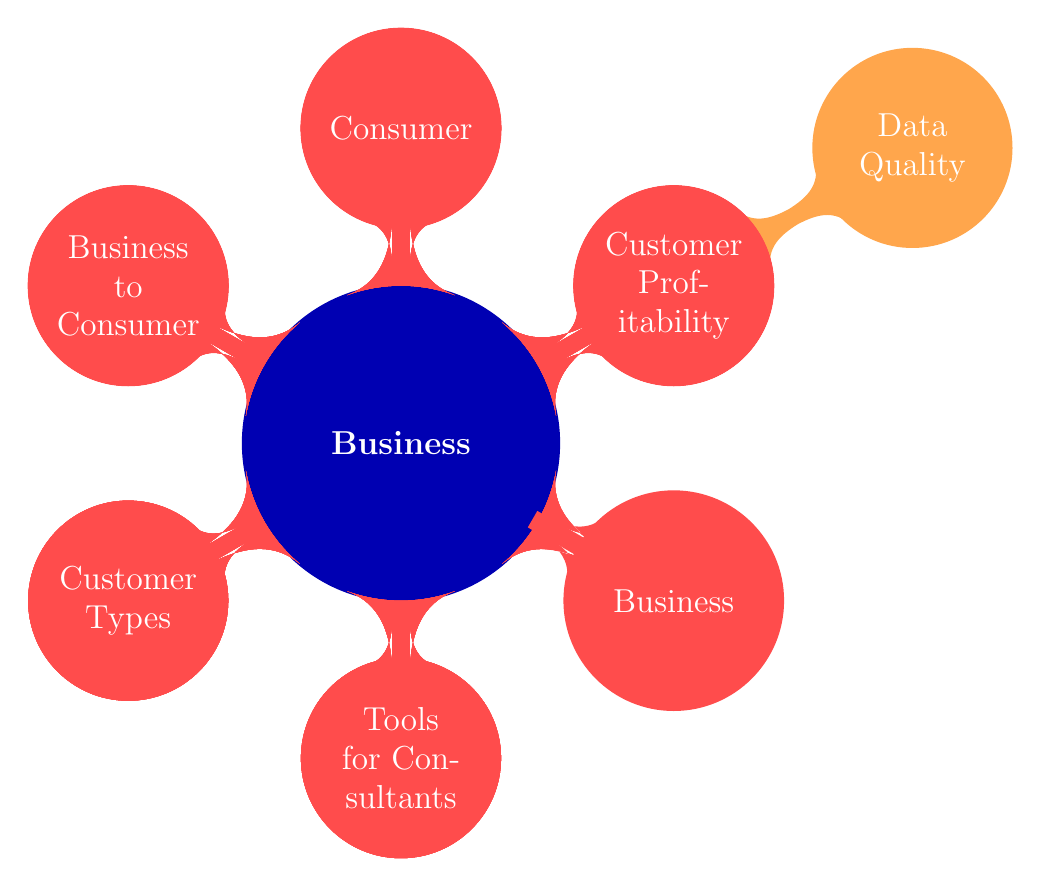
\begin{tikzpicture}[
    mindmap,
    grow cyclic, 
    text=white,
    concept color=blue!70!black, 
    every node/.style={concept, minimum width=2.5cm, align=center, font=\large},
    level 1 concept/.append style={
        level distance=4cm, 
        sibling angle=120, 
        concept color=red!70, 
        font=\Large\bfseries
    },
    level 2 concept/.append style={
        level distance=3.5cm, 
        sibling angle=60, 
        concept color=orange!70,
        font=\large\sffamily
    },
    level 3 concept/.append style={
        level distance=3cm, 
        sibling angle=45, 
        concept color=green!70!black,
        font=\small\sffamily
    },
]

  % START OF TIKZ NODES

  \node[concept] { \textbf{Business} }    child[grow=150] {
        node[concept] {Goals}    } 
    child[grow=30] {
        node[concept] {Make Money}    } 
    child[grow=270] {
        node[concept] {Keep Busy}    } 
    child[grow=210] {
        node[concept] {Share Knowledge}    } 
    child[grow=90] {
        node[concept] {Build Wealth}    } 
    child[grow=330] {
        node[concept] {Address the age discrimination}    } 
    child[grow=150] {
        node[concept] {Our Skills}    } 
    child[grow=30] {
        node[concept] {Data}        child {
            node[concept] {Data Quality}    } } 
    child[grow=270] {
        node[concept] {Data Lineage}    } 
    child[grow=210] {
        node[concept] {Data Science}    } 
    child[grow=90] {
        node[concept] {Data Warehousing}    } 
    child[grow=330] {
        node[concept] {Agile Development}    } 
    child[grow=150] {
        node[concept] {AI	Large Document Analysis}    } 
    child[grow=30] {
        node[concept] {Customer Needs}    } 
    child[grow=270] {
        node[concept] {Reduce Costs}    } 
    child[grow=210] {
        node[concept] {Increase Sales}    } 
    child[grow=90] {
        node[concept] {Writing}    } 
    child[grow=330] {
        node[concept] {Good Ideas}    } 
    child[grow=150] {
        node[concept] {Tax / Spend}    } 
    child[grow=30] {
        node[concept] {AI Book}    } 
    child[grow=270] {
        node[concept] {Data Book}    } 
    child[grow=210] {
        node[concept] {AI Articles}    } 
    child[grow=90] {
        node[concept] {Needs}    } 
    child[grow=330] {
        node[concept] {Funding}    } 
    child[grow=150] {
        node[concept] {Marketing}    } 
    child[grow=30] {
        node[concept] {Customers}    } 
    child[grow=270] {
        node[concept] {Ideas}    } 
    child[grow=210] {
        node[concept] {General Consulting}    } 
    child[grow=90] {
        node[concept] {Sub Contracting}    } 
    child[grow=330] {
        node[concept] {Document Analyzer}    } 
    child[grow=150] {
        node[concept] {True Travel}    } 
    child[grow=30] {
        node[concept] {Customer Profitability}    } 
    child[grow=270] {
        node[concept] {Tools for Consultants}    } 
    child[grow=210] {
        node[concept] {Customer Types}    } 
    child[grow=90] {
        node[concept] {Consumer}    } 
    child[grow=330] {
        node[concept] {Business}    } 
    child[grow=150] {
        node[concept] {Business to Consumer}} 
  ; % End of the main node structure

\end{tikzpicture}

\vspace{0.5in}
\footnotesize
\textit{This mind map was generated from an indented text file using a Python script.}

\newpage
\section*{Mind Map Node Descriptions}
{\centering
\begin{longtable}{@{} p{0.3\textwidth} p{0.6\textwidth} @{}}
    \caption{Node Details and Descriptions} \label{tab:node_details} \\
    \toprule
    \textbf{Node Name} & \textbf{Description} \\
    \midrule
    \endfirsthead

    \multicolumn{2}{c}
    {\normalfont\textbf{\tablename~\thetable\ -- continued}} \\
    \toprule
    \textbf{Node Name} & \textbf{Description} \\
    \midrule
    \endhead
    Business & A business started by Manu and Michael. \\
    \midrule
    Goals & Why do we want to do this? \\
    \midrule
    Make Money &  \\
    \midrule
    Keep Busy &  \\
    \midrule
    Share Knowledge &  \\
    \midrule
    Build Wealth &  \\
    \midrule
    Address the age discrimination &  \\
    \midrule
    Our Skills & What can we do? This is the inside out view. \\
    \midrule
    Data &  \\
    \midrule
    Data Quality &  \\
    \midrule
    Data Lineage &  \\
    \midrule
    Data Science &  \\
    \midrule
    Data Warehousing &  \\
    \midrule
    Agile Development &  \\
    \midrule
    AI	Large Document Analysis &  \\
    \midrule
    Customer Needs & What do our potential customers need? This is the outside in view. \\
    \midrule
    Reduce Costs &  \\
    \midrule
    Increase Sales &  \\
    \midrule
    Writing & Get our message out. \\
    \midrule
    Good Ideas & I have a draft of this book. \\
    \midrule
    Tax / Spend & I have a draft of this book. \\
    \midrule
    AI Book & What would this be? \\
    \midrule
    Data Book & What would this be? \\
    \midrule
    AI Articles & This would be a precursor to our business. \\
    \midrule
    Needs &  \\
    \midrule
    Funding &  \\
    \midrule
    Marketing &  \\
    \midrule
    Customers &  \\
    \midrule
    Ideas &  \\
    \midrule
    General Consulting &  \\
    \midrule
    Sub Contracting &  \\
    \midrule
    Document Analyzer &  \\
    \midrule
    True Travel &  \\
    \midrule
    Customer Profitability &  \\
    \midrule
    Tools for Consultants &  \\
    \midrule
    Customer Types & Which type of customer does our product focus on? \\
    \midrule
    Consumer & A pure consumer product. \\
    \midrule
    Business & A pure business product that is used by a business. \\
    \midrule
    Business to Consumer & A product that is used by businesses to sell to or support consumers. \\
    \midrule
    \bottomrule
\end{longtable}
}


\end{document}
